\section{I. INTRODUCTION}\label{i.-introduction}

\textsc{T}\textsc{HE} relentless evolution toward 6G networks is fundamentally driven by the exponential proliferation of Internet of Things (IoT) ecosystems, which introduces extreme heterogeneity in network traffic and Quality of Service (QoS) requirements\cite{b1}. Modern telecommunication infrastructures must seamlessly accommodate billions of devices with diametrically opposed service profiles over a shared physical substrate\cite{b2}, \cite{b3}. For instance, the Internet of Medical Things (IoMT)---particularly in critical scenarios such as remote robotic surgery, real-time intraoperative diagnostics, and patient telemetry---mandates Ultra-Reliable Low-Latency Communications (URLLC) with deterministic, sub-millisecond response times, absolute data integrity, and extreme fault tolerance\cite{b1}, \cite{b4}, \cite{b5}. In stark contrast, massive urban deployments, such as high-definition Smart City surveillance cameras and immersive extended reality (XR) applications, generate colossal data volumes requiring enhanced Mobile Broadband (eMBB) channels capable of sustaining immense, fluctuating throughput\cite{b4}, \cite{b6}.

Attempting to provision these highly divergent and paradoxical service demands exposes fatal structural limitations in legacy network architectures\cite{b1}, \cite{b7}, \cite{b8}. While traditional Software-Defined Networking (SDN) centralized the control plane to improve programmability and resource abstraction, the reliance on a monolithic controller architecture has proven to be a severe bottleneck in dynamic, large-scale 6G/IoT deployments\cite{b8}, \cite{b9}. Monolithic SDN controllers suffer from inherent scalability constraints, high processing latency, and poor fault isolation, making them wholly incapable of adapting to millisecond-level traffic bursts or handling massive connection densities\cite{b8}, \cite{b9}. Furthermore, the tight, indivisible coupling of internal modules in monolithic systems forces the inefficient replication of the entire controller stack to handle load increases\cite{b8}, \cite{b9}. In high-density IoT environments, this rigid architecture leads to critical single points of failure, unacceptable stochastic queuing delays for time-sensitive IoMT traffic, and severe resource wastage\cite{b9}.

Consequently, overcoming these critical operational bottlenecks makes the adoption of Multi-Tenant Network Slicing, synergized with Microservices-Based SDN architectures, an absolute necessity for isolated orchestration\cite{b8}, \cite{b9}. Network slicing allows operators to logically partition the shared physical infrastructure into customized, end-to-end virtual networks, ensuring that the massive bandwidth demands of Smart City cameras are perfectly isolated from the life-critical latency pathways required by surgical IoMT slices\cite{b1}, \cite{b2}. To achieve the granular agility and resilience required for this dynamic slice orchestration, the industry is decomposing the monolithic SDN control plane into decentralized, loosely coupled microservices deployed within lightweight container platforms like Kubernetes\cite{b8}, \cite{b10}. This microservices-driven decomposition enables independent scaling, rapid service deployment, and robust fault containment, establishing the indispensable architectural foundation for autonomous, secure resource orchestration in next-generation 6G environments\cite{b8}.

The disaggregation of control plane functionalities into loosely coupled microservices injects severe orchestration complexity and substantial inter-service latency overhead into the network fabric\cite{b11}. In high-density IoT deployments, the continuous intra-cluster communication between containerized virtual network functions, exacerbated by virtualization overhead and dynamic resource contention, creates an unpredictable, highly stochastic queuing environment at the data plane\cite{b12}. Static heuristic policies and reactive, rule-based orchestrators fundamentally lack the predictive agility and continuous control resolution required to navigate such complex state transitions, leading inevitably to severe resource mismanagement or catastrophic Service Level Agreement (SLA) violations across critical network slices\cite{b13}.

Although Deep Q-Networks (DQN) have proven capable of improving the throughput of edge computing resource allocation\cite{b14}, \cite{b15}, these algorithms suffer from a fundamental weakness in the form of overestimation bias and limitations in discrete action spaces that hinder the precision of continuous bandwidth slicing. Mitigation efforts using the Dueling Double DQN (D3QN) architecture have indeed succeeded in stabilizing learning in latency-critical environments such as URLLC and maritime IoT\cite{b13}, \cite{b16}. However, D3QN still operates with discrete actions that are mathematically irrelevant for adjusting container resource capacity (sizing), which demands high granularity within microservices architectures.

As a solution to the limitations of discrete control, Proximal Policy Optimization (PPO) offers continuous control that is architecturally superior, particularly for maintaining spectrum stability in Healthcare IoT\cite{b17}. PPO's advantage lies in its trust region clipping mechanism, which strictly prevents agent policy updates from disrupting network services. Although promising high precision, this algorithm is highly prone to convergence failures and requires the integration of complex reward shaping mechanisms to enable agents to adapt optimally within highly dynamic multi-tenant operational environments\cite{b18}.

Despite these algorithmic advancements, there is a critical operational gap that exposes a major weakness in the existing literature. The majority of current DRL studies for network slicing are exclusively validated using software simulations (such as NS-3) under the assumption of generic network parameter\cite{b15}-\cite{b20}. This theoretical approach fatally overlooks real-world anomalies---such as queuing delays, communication latency overhead, and CPU resource contention---which absolutely disrupt hardware-based Edge infrastructure and Kubernetes/microservices orchestration. These AI policies, which only converge on paper, are bound to fail in responding to the volatility of real-world physical deployments; a critical architectural gap that is the primary focus of this research.

To bridge the operational gap between theoretical simulation and physical deployment, this research introduces SDH-PPO (Safe-Driven Hybrid Proximal Policy Optimization), an advanced reinforcement learning framework engineered specifically for microservices-based SDN orchestration. SDH-PPO serves as the ultimate solution to microservices volatility by uniquely employing a hybrid action space, empowering the AI agent to simultaneously execute discrete network port selections and formulate precise, continuous bandwidth allocations in real-time. Furthermore, to overcome the convergence failures caused by static training datasets and unreferenced functions, the framework integrates an Enhanced Optimization Wasserstein Generative Adversarial Network (EO-WGAN) to synthesize extreme network variance, proactively exposing the agent to latency anomalies prior to deployment.

The primary contributions of this paper are explicitly defined as follows:

\begin{itemize}
\item
  Design a novel SDH-PPO framework to dynamically orchestrate resources across heterogeneous, multi-tenant IoT slices.
\item
  Formulate a mathematical Safety Layer based on action projection to proactively override destructive agent decisions.
\item
  Construct microservices-based SDN architecture by containerizing Ryu controller to enforce stringent and scalable network slice isolation.
\item
  Construct a robust multi-tenant network slicing environment to dynamically enforce differentiated Quality of Service (QoS) requirements, ensuring strict resource isolation and tailored performance guarantees across competing service tenants.
\item
  Implement the proposed orchestration framework on edge computing testbed powered by Raspberry Pi 5, transitioning from generic software simulations to real-world physical deployments.
\end{itemize}

\section{II. Related Work}\label{ii.-related-work}

\subsection{A. Architectural Evolution: From Monolithic SDN to Microservices-Based Slicing}\label{a.-architectural-evolution-from-monolithic-sdn-to-microservices-based-slicing}

The architectural evolution from monolithic Software-Defined Networking (SDN) infrastructures to service-based microsegmentation represents a structural imperative for scaling heterogeneous networks, yet the literature exposes a stark dialectical tension between theoretical decentralization and operational bloat. Traditional optimization strategies primarily focus on the physical distribution of logically centralized controllers to mitigate latency; for instance, Abderrahmane et al. tackle the Controller Placement Problem (CPP) using heuristic meta-algorithms to optimize physical topology\cite{b19}. However, this spatial distribution approach merely replicates entire monolithic control stacks across nodes, inherently suffering from severe code inefficiency and failing to address underlying architectural rigidities\cite{b8}, \cite{b19}.

To overcome this, recent frameworks advocate for fundamentally disaggregating the control plane into independent microservices. Arzo et al. and Sharma demonstrate that transitioning to Cloud-Native Network Functions (CNFs) by decomposing monolithic controllers into Kubernetes-orchestrated containers enhances agility, allows for independent lifecycle management, and improves resource density\cite{b8}, \cite{b10}. Nevertheless, these cloud-native transitions expose severe methodological weaknesses. Sharma critically notes an overestimation bias in deployment readiness, highlighting a fundamental friction between the strictly stateful nature of telecom workloads (e.g., session management and subscriber tracking) and Kubernetes' inherently stateless design assumptions\cite{b10}.

While containerized microsegmentation theoretically optimizes resource isolation, empirical evaluations consistently reveal prohibitive orchestration latencies that undermine Quality of Service (QoS). Fernandez et al. and Botez et al. leverage Kubernetes to orchestrate IoT slices across distributed micro-edge and cloud boundaries, positing that such multi-tier architectures guarantee high availability and traffic isolation\cite{b20}, \cite{b21}. Yet, a critical synthesis of their findings exposes the operational bottlenecks introduced by the orchestrator itself. Botez et al. demonstrate that relying on default Kubernetes Horizontal Pod Autoscalers (HPA) creates profound orchestration delays---often spanning several seconds during SLA violations---because the orchestration engine struggles to rapidly process and react to external network metrics\cite{b20}. Attempting to bypass these top-heavy orchestration delays, Holscher embeds the microservice orchestration logic directly into the SDN data plane using switches\cite{b21}. Paradoxically, while this mitigates baseline latency for pre-established routes, Holscher's methodology exposes a fatal scalability flaw: flow-table misses force requests through the centralized controller, exacerbating worst-case tail latencies by several orders of magnitude and rendering the architecture highly vulnerable to the bursty, unpredictable traffic typical of massive IoT deployments\cite{b21}.

\begin{table*}[t]
\centering
\caption{State-of-the-Art Comparison of DRL-Based Orchestration Frameworks for SDN-IoT Networks}
\label{tab:1}
\scriptsize
\begin{tabular}{lccccccc}
\toprule
Reference & Hybrid/Action Space & Ratio Sizing & Multi Tenant Slicing & Microservices Isolation & Generative Augmentation & Strict Priority SLA Penalty & Physical Validation \\
\midrule
Proposed & \checkmark & \checkmark & \checkmark & \checkmark & \checkmark & \checkmark & \checkmark \\
\cite{b22} & - & - & \checkmark & - & - & - & - \\
\cite{b23} & - & - & \checkmark & - & - & \checkmark & - \\
\cite{b24} & - & - & - & \checkmark & - & \checkmark & \checkmark \\
\cite{b25} & - & - & \checkmark & - & - & - & \checkmark \\
\cite{b26} & - & - & \checkmark & - & - & - & - \\
\cite{b8} & - & - & - & \checkmark & - & - & - \\
\cite{b27} & \checkmark & \checkmark & \checkmark & - & - & - & - \\
\cite{b28} & - & - & \checkmark & - & - & - & - \\
\cite{b10} & - & - & \checkmark & \checkmark & - & - & - \\
\cite{b4} & \checkmark & \checkmark & \checkmark & - & \checkmark & - & - \\
\cite{b29} & \checkmark & \checkmark & - & - & - & - & - \\
\cite{b30} & - & - & \checkmark & - & - & - & - \\
\cite{b31} & - & - & - & \checkmark & - & - & - \\
\cite{b32} & - & - & \checkmark & - & - & - & - \\
\cite{b33} & - & - & \checkmark & - & - & - & - \\
\cite{b34} & - & - & \checkmark & - & \checkmark & - & - \\
\cite{b35} & - & - & \checkmark & - & - & - & \checkmark \\
\cite{b20} & - & - & \checkmark & \checkmark & - & - & \checkmark \\
\cite{b3} & - & - & \checkmark & - & - & - & - \\
\cite{b9} & - & - & - & \checkmark & - & - & \checkmark \\
\cite{b17} & - & - & \checkmark & - & - & - & - \\
\cite{b6} & \checkmark & \checkmark & \checkmark & - & - & - & - \\
\cite{b36} & - & - & \checkmark & - & - & - & - \\
\cite{b14} & - & - & \checkmark & - & - & - & - \\
\cite{b37} & - & - & - & \checkmark & - & - & - \\
\bottomrule
\end{tabular}
\\[2pt]
\footnotesize{*Notes: (\checkmark) indicates the implementation of advanced architecture/algorithm corresponding to the specific column feature; (-) indicates the use of legacy methods, discrete approximations, static environments, unconstrained exploration, or software-only simulations.}
\end{table*}

Furthermore, the structural decomposition of SDN into service-based microsegments exponentially expands the attack surface and complicates Service Function Chaining (SFC), prompting the integration of security mechanisms that inadvertently cripple network agility. Zhang et al. correctly identify that the tight coupling of traditional SFCs causes deployment gridlocks and service collisions, proposing an Artificial Intelligence (AI)-driven demand management model secured by consortium blockchains\cite{b21}. However, this methodology exemplifies a persistent theoretical blindness to real-time performance constraints. By strictly imposing Diffie-Hellman key exchanges and distributed ledger consensus for microservice identity authentication, Zhang et al. introduce massive computational overheads that directly negate the lightweight, low-latency benefits of the microservice architecture they aim to optimize\cite{b38}. Ultimately, while the literature confirms that migrating from monolithic controllers to service-based microsegmentation resolves macroscopic scalability limitations\cite{b8}, \cite{b12}, \cite{b19}.

\subsection{B. Limitations of Value-Based Algorithms in Resource Orchestration}\label{b.-limitations-of-value-based-algorithms-in-resource-orchestration}

The transition toward intelligent resource orchestration in Software-Defined Networking (SDN) and IoT environments has been heavily driven by first-generation value-based Deep Reinforcement Learning (DRL) algorithms. Early implementations of Q-Learning and Deep Q-Networks (DQN) successfully demonstrate the capacity to enhance network throughput and minimize latency by dynamically mapping network states to resource provisioning actions. For instance, Alrifai et al. established that utilizing a DQN-based approach for 5G resource allocation yields up to a 25.7\% improvement in aggregate throughput and a 31.5\% reduction in latency compared to traditional heuristic models\cite{b14}. This capacity for optimizing fundamental network parameters is corroborated by Hosseinzadeh et al., who applied DQN to multi-objective resource allocation scenarios in edge computing, proving its empirical efficacy in decentralizing workloads and reducing operational service delays\cite{b15}.

Despite these substantial throughput and latency improvements, first-generation DQN architectures suffer from critical algorithmic flaws that hinder their effectiveness in highly dynamic environments: overestimation bias and discrete action spaces. Standard DQN relies on the same neural network weights to both select and evaluate the maximum action value, frequently resulting in overly optimistic value estimations. As Xu et al. highlight, this action selection bias and overestimation can cause the algorithm to become unstable, leading to erratic resource allocation decisions during network fluctuations\cite{b13}. Furthermore, Onaji et al. argue that modeling resource orchestration through discrete action spaces inherently lacks the granularity required to perform fine-grained resource adjustments, leading to coarse block allocations that waste resources\cite{b6}.

To combat the instability and overestimation bias of standard DQN, the literature showcases a definitive algorithmic evolution toward Dueling Double DQN (D3QN) architectures. By decoupling the value function into a state-value stream and an advantage-function stream, D3QN enables the agent to evaluate the utility of network states independently from the actions themselves. Xu et al. leveraged this dual-network architecture to optimize computation offloading in maritime IoT, proving that D3QN effectively resolves the overestimation problem and converges to optimal strategies significantly faster and more stably than standard DQN\cite{b13}. Building upon this, recent literature introduces Reinforced Dueling Deep Q-Networks (RDDQN) for 5G URLLC congestion control, embedding ultimatum game-theoretic mechanisms into the dueling architecture to stabilize delay fairness and accelerate decision latency to sub-millisecond levels\cite{b16}.

However, the application of these advanced value-based methods in modern containerized infrastructures reveals a fatal mathematical paradox. While D3QN and its advanced variants successfully stabilize convergence and mitigate overestimation bias, they remain fundamentally locked into discrete action spaces\cite{b13}. Orchestrating network slices across containerized microservices is not a discrete problem; managing container bandwidth and CPU quotas requires fluid, continuous percentage allocation to strictly adhere to dynamic Quality of Service (QoS) boundaries\cite{b6}, \cite{b39}. Because D3QN mathematically forces these continuous bandwidth requirements into predefined, quantized categorical actions, it is inherently flawed for precise container orchestration\cite{b6}. As emphasized by Onaji et al., this rigid discrete quantization prevents the exact, fractional scaling necessary for microservices, forcing larger, imprecise adjustments that cause transient overshoots and ultimately degrade the QoS of critical network slices\cite{b6}.

\subsection{C. The Potential and Limitations of Policy-Gradient (PPO)}\label{c.-the-potential-and-limitations-of-policy-gradient-ppo}

To overcome the fundamental limitations of discrete action spaces inherent in first-generation value-based methods, recent literature has pivoted toward policy-gradient algorithms to manage the fluid demands of network slicing. For continuous control tasks---such as the hybrid bandwidth allocation required for orchestrating containerized microservices---Proximal Policy Optimization (PPO) has emerged as the state-of-the-art solution. Unlike its predecessors, PPO directly optimizes the control policy while maintaining operational stability through a unique mathematical constraint. As Abdulazeez et al. detail, PPO introduces a clipped surrogate objective function---an evolution of Trust Region Policy Optimization (TRPO)---which explicitly restricts how much the decision-making policy is permitted to change during a single training update\cite{b40}.

In the context of Software-Defined Networking (SDN) infrastructure, this trust region clipping acts as a critical structural safeguard. Chahoud et al. emphasize that without this clipping mechanism, extreme policy updates could completely destabilize the network controller, leading to erratic resource provisioning and catastrophic network damage\cite{b18}. By constraining the probability ratio of the policy updates, PPO ensures that continuous adjustments to CPU quotas and bandwidth percentages remain safe, smooth, and bounded. This allows the physical infrastructure to respond to IoT traffic spikes without overshooting critical boundaries or severely degrading the network\cite{b18}. This capability is firmly corroborated by Hosseinzadeh et al., who highlight the effectiveness of PPO in executing dynamic, continuous task scheduling across heterogeneous edge computing nodes to seamlessly balance physical network loads\cite{b15}.

However, deploying standard PPO in highly dynamic, containerized environments exposes a critical architectural vulnerability. While the clipping mechanism guarantees safe updates, the standard PPO algorithm is notoriously sample-inefficient\cite{b18}. Alrifai et al. argue that in environments characterized by non-stationary traffic and high IoT mobility, reinforcement learning agents suffer from delayed feedback and the exponential growth of continuous state-action spaces, which severely cripples their exploration efficiency\cite{b14}. This sample inefficiency becomes a fatal flaw when applied to fluctuating microservices topologies. Sittakul et al. demonstrate that standard policy-gradient allocators like PPO converge sluggishly when faced with the high-dimensional state spaces of modern 5G infrastructure\cite{b16}.

The climax of this algorithmic limitation lies in the extreme volatility of the microservices themselves. In an environment where IoT slice demands and container deployments fluctuate by the millisecond, standard PPO simply cannot gather and process interaction data fast enough. Chahoud et al. highlight this paradox: by the time standard PPO eventually converges on an optimal continuous allocation strategy, the underlying network state has already shifted, rendering the newly learned policy entirely obsolete\cite{b18}. Because it fails to converge fast enough to keep pace with rapid environmental changes, standard PPO inevitably degrades the Quality of Service (QoS) for critical network slices. Consequently, the literature indicates that standard PPO, despite its superior continuous control mechanisms, is inherently insufficient for modern SDN orchestration on its own. To prevent convergence failures and overcome severe sample inefficiency, PPO strictly necessitates the integration of auxiliary acceleration mechanisms---such as advanced reward shaping or robust data augmentation---to viably function within rapidly fluctuating microservices architectures\cite{b18}.

\section{III. Method}\label{iii.-method}

The methodology of this research is structured to facilitate an autonomous and adaptive resource orchestration within a multi-tenant SDN environment. The framework logic is divided into system architecture, data augmentation, and the deep reinforcement learning optimization process.

\subsection{A. Environment Architecture}\label{a.-environment-architecture}

The system is designed as a multi-tenant SDN-based framework that enables end-toend network slicing for heterogeneous IoT applications. The architecture facilitates the flow of telemetry data from the physical perception layer to a partitioned storage environment, overseen by a hierarchical control plane that ensures strict tenant isolation.

\begin{enumerate}
\def\labelenumi{\arabic{enumi})}
\item
  \textbf{Data Acquisition and IoT Gateways}
\end{enumerate}

At the physical layer, real-time data is captured by various sensor nodes deployed across different operational sectors. Each sector utilizes a Raspberry Pi gateway to aggregate these raw readings and encapsulate them into a standardized JSON format for transmission. This setup includes healthcare sensors for monitoring SpO2 and heart rates, camera-based vision sensors for smart city human detection, and environmental sensors for smart building telemetry such as humidity and temperature.

\begin{figure}[htbp]
\centering
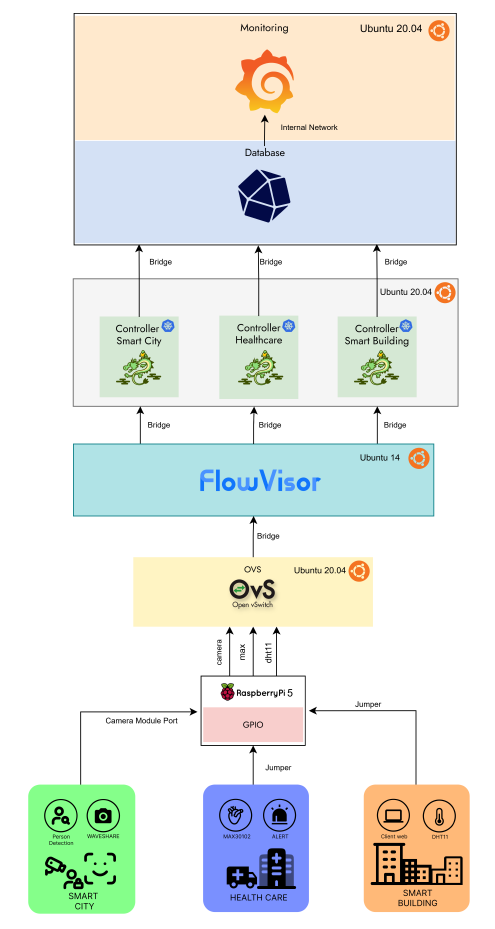
\includegraphics[width=\columnwidth]{figures/fig1_architecture.png}
\caption{SDN IoT Architecture.}
\label{fig:1}
\end{figure}


\begin{enumerate}
\def\labelenumi{\arabic{enumi})}
\setcounter{enumi}{1}
\item
  \textbf{Network Slicing and Service Requirements}
\end{enumerate}

To accommodate the diverse performance needs of each sector, the network is logically partitioned into three distinct slices. Each slice is configured with specific parameters to meet its operational objectives:

\begin{itemize}
\item
  \emph{Slice 1 (Healthcare Sector)}. This slice handles critical medical telemetry. Given the sensitivity of physiological data, it is assigned the highest priority in the network. The configuration focuses on achieving ultra-low latency and minimal jitter to support real-time health monitoring and emergency response.
\item
  \emph{Slice 2 (Smart City Sector)}. Dedicated to multimedia and vision-based data, this slice manages high-volume traffic from camera sensors. Its primary requirement is high bandwidth availability, ensuring that metadata and image streams can be transmitted with sufficient throughput for accurate presence detection.
\item
  \emph{Slice 3 (Smart Building Sector)}. This partition manages environmental monitoring data. Because humidity and temperature changes occur over longer intervals, the slice is treated as low-priority or best-effort traffic. It is designed to be more tolerant of latency, allowing the network to prioritize resources for the more time-critical slices.
\end{itemize}

\begin{enumerate}
\def\labelenumi{\arabic{enumi})}
\setcounter{enumi}{2}
\item
  \textbf{Control Plane and Tenant Isolation}
\end{enumerate}

The orchestration between these slices is managed by a transparent proxy layer using Flowvisor, which resides between the Open vSwitch (OvS) and the controller instances. Flowvisor inspects incoming packets at the switch ports and applies FlowSpace rules to ensure traffic is correctly mapped to the corresponding tenant.

Each slice is governed by an independent Ryu Controller instance. Once the Flowvisor identifies the packet's origin, it redirects the request to the specific Ryu Controller responsible for that tenant. The controller then provides the necessary flow instructions back to the OvS, which subsequently routes the JSON-formatted data into isolated database buckets. This mechanism ensures that data from the healthcare sector remains strictly separated from smart city or building data. Finally, the entire performance of the network, including the health of each individual slice, is monitored and visualized in real-time through a Grafana dashboard.

\subsection{B. Augmentation}\label{b.-augmentation}

The data initialization phase utilizes a Gaussian Noise Injection technique, as formally described in Equation 1. This procedure integrates additive noise, where \(\epsilon \sim N(0,0.5)\), into the input space primarily to mitigate training instabilities and prevent the occurrence of mode collapse. This approach aligns with the stabilization principles proposed by Arjovsky for Generative Adversarial Networks (GANs), ensuring model convergence even when real and synthetic data distributions exhibit minimal overlap\cite{b41}. Furthermore, the injection of Gaussian noise serves as a robust data augmentation strategy for Reinforcement Learning (RL) agents; by introducing variance into state representations, the model achieves enhanced environmental diversity and improved generalization capabilities. The specific selection of a 0.5 standard deviation was determined through empirical hyperparameter tuning, specifically tailored to the normalization scale of the research dataset.

\begin{equation}\label{eq:1}
x_{noisy} = x_{real} + \epsilon,\quad\epsilon \sim \mathcal{N}\left( 0,\sigma^{2} \right)\
\end{equation}

The Critic's objective function, formulated in Equation 2, minimizes theWasserstein distance between real and generated data distributions to enhance discriminative precision while ensuring training stability. To enforce the 1-Lipschitz continuity constraint, a gradient penalty term is integrated to penalize the L2 norm of the gradient with respect to interpolated samples when it deviates from unity.

\begin{equation}\label{eq:2}
L_{D} = \mathbb{E}_{\widetilde{\mathbb{x}} \sim \mathbb{P}_{\mathbb{g}}}\left\lbrack D\left( \widetilde{x} \right) \right\rbrack - \mathbb{E}_{\mathbb{x} \sim \mathbb{P}_{\mathbb{r}}}\left\lbrack D(x) \right\rbrack + \lambda\mathbb{E}_{\widehat{\mathbb{x}} \sim \mathbb{P}_{\widehat{\mathbb{x}}}}\left\lbrack \left( \text{|}\nabla_{\widehat{x}}D\left( \widehat{x} \right)\text{|}_{2} - 1 \right)^{2} \right\rbrack
\end{equation}

The Generator's objective function, as defined in Equation 3, is formulated to minimize the negative expectation of the scores assigned by the Critic to synthetic samples. By minimizing this loss, the Generator is effectively trained to maximize the perceived authenticity of its output, thereby producing synthetic data that is indistinguishable from the real data distribution to deceive the Critic.

\begin{equation}\label{eq:3}
L_{G} = - \mathbb{E}_{\widetilde{\mathbb{x}} \sim \mathbb{P}_{\mathbb{g}}}\left\lbrack D\left( \widetilde{x} \right) \right\rbrack
\end{equation}

The data interpolation step, as expressed in Equation 4, generates intermediate samples \(\widehat{x}\) by linearly combining real and generated data with a random scaling factor \(\alpha \sim U(0,1)\). This interpolation is essential for calculating the gradient penalty, as it allows the model to enforce the 1-Lipschitz constraint by penalizing the Critic's gradient norm along the path between the real and synthetic data distributions.

\begin{equation}\label{eq:4}
\widehat{x} = \alpha x + (1 - \alpha)\widetilde{x},\quad\alpha \sim \text{U}(0,1)
\end{equation}

The bandwidth utilization metric, as formulated in Equation 5, calculates the percentage of consumed throughput relative to the maximum policing rate by normalizing received traffic into a consistent unit of measurement. This equation ensures a precise mathematical correlation between actual data flow and the bandwidth constraints enforced by the SDN controller, thereby facilitating accurate monitoring of network resource consumption.

\begin{equation}\label{eq:5}
U = \left( \frac{RX_{mbps} \times 1000}{Policing_{kbps}} \right) \times 100
\end{equation}

\begin{equation}\label{eq:6}
D = \left\{ \begin{array}{r}
\frac{\left( {RX}_{mbps} \times 1000 \right) - {Policing}_{kbps}}{80},if\left( {RX}_{mbps} \times 1000 \right) > {Policing}_{kbps} \\
0,\ \ otherwise
\end{array} \right.\
\end{equation}

The packet drop logic, as defined in Equation 6, functions as a deterministic model for the SDN traffic policing mechanism by calculating the volume of discarded packets when ingress traffic exceeds the prescribed bandwidth threshold. By incorporating a constant divisor of 80 to approximate average packet sizes, the formula effectively converts the excess bitrate into a discrete packet loss count, thereby maintaining mathematical consistency between throughput and drop metrics in the synthetic dataset.

\subsection{C. Pre-Processing}\label{c.-pre-processing}

The sigmoid penalty function, as defined in Equation 7, serves as a risk-sensitive soft constraint that penalizes the agent based on the proximity of network latency to the Service Level Agreement (SLA) threshold. By providing a continuous gradient controlled by the steepness parameter \(k\), this mechanism allows the PPO agent to proactively adjust resource allocation as latency nears the critical limit \(\tau\), thereby preventing abrupt performance degradation.

\begin{equation}\label{eq:7}
P_{lat}(v,\tau,k) = \frac{1}{1 + e^{- k(v - \tau)}}
\end{equation}

The throughput incentive, as defined in Equation 8, assesses the fulfillment of bandwidth requirements by calculating the ratio between the actual received throughput and the target capacity for Port 2. By implementing a clipping mechanism to bound the reward within the \(\lbrack 0,1\rbrack\) interval, the function prevents greedy resource consumption and promotes balanced allocation across other network ports once the target is satisfied.

\begin{equation}\label{eq:8}
R_{thr} = \text{clip}\left( \frac{RX_{p2}}{T_{p2}},0,1 \right)
\end{equation}

The global reliability penalty, as defined in Equation 9, quantifies network unreliability by aggregating packet drops across all slices and normalizing the total against an empirical threshold of 50. This mechanism discourages the agent from assigning policing rates that exceed physical link capacities, thereby mitigating the risk of mass congestion and systemic packet loss within the Open vSwitch (OVS) infrastructure.

\begin{equation}\label{eq:9}
P_{drop} = \text{clip}\left( \frac{\sum_{i \in \text{\{}1,2,4\text{\}}}^{}{Drop_{pi}}}{50},0,1 \right)
\end{equation}

The total reward function, as formulated in Equation 10, integrates multiple incentives and penalties into a unified scalar signal to guide the Deep Reinforcement Learning (DRL) agent's optimization process. By assigning the highest weight coefficient to the latency penalty of the healthcare slice (\(P_{lat\text{\_}p4}\)), the formulation enforces a priority-aware strategy that prioritizes critical delay requirements over throughput maximization and global network stability.

\begin{equation}\label{eq:10}
R_{total} = \left( 0.4 \times R_{thr} \right) - \left( 0.6 \times P_{lat\text{\_}p4} \right) - \left( 0.2 \times P_{drop} \right)
\end{equation}

The continuous action space within the SDH-PPO framework is defined in Equation 11 as the relative ratio of change in the policing rate to facilitate stable and incremental network resource adjustments. This ratio-based approach is preferred over absolute value estimation to ensure that policy updates remain within the PPO algorithm\textquotesingle s trust-region constraints, thereby improving training convergence and operational stability.

\begin{equation}\label{eq:11}
a_{cont} = \frac{\rho_{t + 1} - \rho_{t}}{\rho_{t}}
\end{equation}

\begin{equation}\label{eq:12}
z = \frac{x - \mu}{\sigma}
\end{equation}

The Z-score standardization method, as formulated in Equation 12, transforms input features to follow a normal distribution with a mean of zero and a variance of one. This pre-processing procedure is critical for balancing the contributions of features with heterogeneous scales, thereby preventing gradient dominance by large numerical values and ensuring training stability for the PPO agent.

\subsection{D. Proposed Framework}\label{d.-proposed-framework}

The proposed framework consists of four primary internal components that work synchronously to achieve optimal policy convergence:

\begin{itemize}
\item
  Actor Network (\(\pi_{\theta}\)): Responsible for the decision-making process. It maps the high-dimensional state space \(s_{t}\) into a continuous action space \(a_{t}\), representing the optimal resource allocation or policing rate.
\item
  Critic Network (\(V_{\phi}\)): Acts as the evaluator by estimating the state-value function \(V\left( s_{t} \right)\). It provides a baseline to calculate the advantage signal, which guides the Actor\textquotesingle s learning process.
\item
  Experience Replay Buffer: A temporal storage unit that collects trajectories \(\tau = \left( s_{t},a_{t},r_{t},s_{t + 1} \right)\). Unlike off-policy methods, this buffer is used to store mini-batches for the PPO\textquotesingle s stochastic gradient descent (SGD) updates before being cleared for the next iteration.
\item
  PPO Update Engine: The central computational unit that executes the Clipped Surrogate Objective and Generalized Advantage Estimation (GAE) to update the networks\textquotesingle{} weights without causing destructive policy shifts.
\end{itemize}

\begin{enumerate}
\def\labelenumi{\arabic{enumi})}
\item
  \textbf{Mathematical Formulation}
\end{enumerate}

To ensure training stability, the proposed framework implements the following mathematical constraints:

\begin{itemize}
\item
  \textbf{Clipped Objective Function:} To prevent excessively large policy updates, the Actor is optimized by maximizing the clipped surrogate objective:
\end{itemize}

\begin{equation}\label{eq:13}
L^{CLIP}(\theta) = \widehat{\mathbb{E}_{t}}\left\lbrack \min\left( r_{t}(\theta)\widehat{A_{t}},\text{clip}\left( r_{t}(\theta),1 - \epsilon,1 + \epsilon \right)\widehat{A_{t}} \right) \right\rbrack
\end{equation}

where \(r_{t}(\theta)\) is the probability ratio:

\begin{equation}\label{eq:14}
r_{t}(\theta) = \frac{\pi_{\theta}\left( a_{t} \middle| s_{t} \right)}{\pi_{\theta_{old}}\left( a_{t} \middle| s_{t} \right)}
\end{equation}

\begin{itemize}
\item
  \textbf{Advantage Estimation:} We employ Generalized Advantage Estimation (GAE) to reduce variance during training:
\end{itemize}

\begin{equation}\label{eq:15}
\widehat{A_{t}} = \delta_{t} + (\gamma\lambda)\delta_{t + 1} + \ldots + (\gamma\lambda)^{T - t + 1}\delta_{T - 1}
\end{equation}

where \(\delta_{t} = r_{t} + \gamma V_{\phi}\left( s_{t + 1} \right) - V_{\phi}\left( s_{t} \right)\ \)represents the Temporal Difference (TD) error.

\begin{figure}[htbp]
\centering
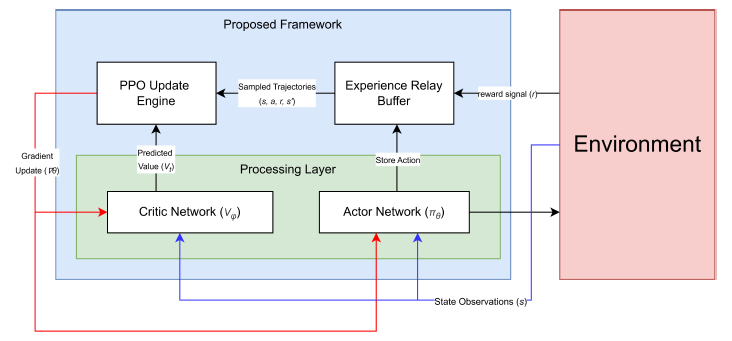
\includegraphics[width=\columnwidth]{figures/fig2_framework.png}
\caption{SDH-PPO Framework.}
\label{fig:2}
\end{figure}


\begin{enumerate}
\def\labelenumi{\arabic{enumi})}
\setcounter{enumi}{1}
\item
  \textbf{Algorithmic Logic Flow}
\end{enumerate}

The interaction between the proposed agent and the target environment follows a strictly defined logical sequence:

\begin{itemize}
\item
  \textbf{Interaction Phase}: The environment transmits the state observation \(s_{t}\) to the Actor and Critic. The Actor generates an action \(a_{t}\), which is executed in the environment, resulting in a reward \(r_{t}\) and the next state \(s_{t + 1}\).
\item
  \textbf{Data Collection}: The transition tuple \(\left( s_{t},a_{t},r_{t},s_{t + 1} \right)\) is stored in the Experience Replay Buffer.
\item
  \textbf{Optimization Phase}: The Update Engine samples a mini-batch of trajectories from the buffer and fetches the predicted value \(V_{t}\) from the Critic Network to compute the loss.
\item
  \textbf{Weight Convergence}: The engine computes the gradients \(\nabla\theta\) and \(\nabla\phi\), initiating a backpropagation process to update the weights of both the Actor and Critic networks, respectively.
\end{itemize}

\subsection{E. Model Comparison}\label{e.-model-comparison}

The performance of the proposed SDH-PPO framework is evaluated through a comparative analysis against several state-of-the-art reinforcement learning models and traditional benchmarks. To ensure a rigorous and scientifically valid assessment, five distinct architectural approaches are examined: the Deep Q-Network (DQN), Double DQN (DDQN), Proximal Policy Optimization (PPO), our introduced SDH-PPO framework, and a non-AI static heuristic baseline. As summarized in Table 2, a standardized set of global hyperparameters is uniformly applied to all learning agents to mitigate performance biases arising from optimization variances. All reinforcement learning (RL) models undergo training for 2,000 epochs utilizing the Adam optimizer with a learning rate of 0.0003 and a batch size of 64. Furthermore, the discount factor (\(\gamma\)) is strictly maintained at 0.99 to encourage the agents to prioritize long-term Service Level Agreement (SLA) fulfillment over immediate rewards. To provide equivalent representational power across all models, each neural network architecture is standardized with a capacity of 256 hidden units.

The implementation of these parameters varies according to the structural requirements of each framework while remaining strictly within the defined constraints. For value-based methods such as DQN and DDQN, the 256-neuron hidden layers map the 37 state features to discrete action values, whereas the actor-critic architectures of PPO and the proposed SDH-PPO distribute this neural capacity to manage continuous and hybrid action spaces, respectively. By subjecting the proposed SDH-PPO framework to these uniform settings---including the standardized learning rate and batch size---the experiment validates that any significant reduction in SLA violations is a direct consequence of its specialized Dueling and Safety Layer architecture rather than advantageous training parameters. Finally, the static heuristic baseline is evaluated over the same 2,000 simulation steps using a \(\gamma\) of 0.99, establishing a performance lower bound to highlight the adaptive superiority of the AI-driven approaches in dynamic Software-Defined Networking (SDN) environments.

\begin{table}[htbp]
\centering
\caption{Hyperparameter Settings}
\label{tab:2}
\begin{tabular}{cccccc}
\toprule
Epochs & LR & Batch Size & Optimizer & $\gamma$ & Hidden Layers \\
\midrule
2000 & 0.0003 & 64 & Adam & 0.99 & 256 \\
\bottomrule
\end{tabular}
\end{table}

\section{IV. Result}\label{iv.-result}

The performance evaluation demonstrates the efficacy of the SDH-PPO framework in dynamic network slicing scenarios. The experimental results, including comparisons against state-of-the-art models, are summarized in Table 3.

\subsection{A. Augmentation}\label{a.-augmentation}

The representational accuracy and structural integrity of the generated synthetic dataset are validated through a high-dimensional feature visualization, as manifested in Fig.3. The resulting visualization exhibits a substantial overlap and a synchronized density distribution between the original and augmented data points throughout the feature space. This high degree of stochastic alignment confirms that the generative framework specifically the Wasserstein Generative Adversarial Network with Gradient Penalty (WGAN-GP) has effectively encapsulated the latent probability distributions inherent in real-world IoT network traffic. While the overlapping clusters serve as a proxy for high data fidelity, the broad spatial distribution ensures that the augmented samples provide the necessary diversity for robust training. Such characteristics are instrumental in fortifying the PPO agent against overfitting to restricted historical observations, thereby enhancing its generalization capabilities across a wide array of dynamic network slicing scenarios.

\begin{figure}[htbp]
\centering
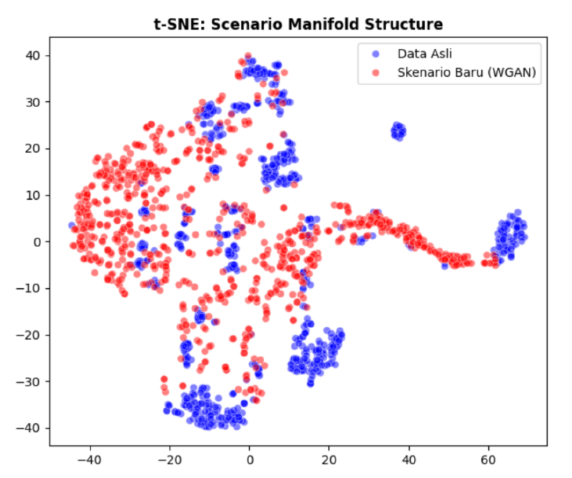
\includegraphics[width=\columnwidth]{figures/fig3_tsne.png}
\caption{t-SNE Visualization.}
\label{fig:3}
\end{figure}


\subsection{B. Model Evaluation}\label{b.-model-evaluation}

The training dynamics and convergence behavior of the evaluated models are illustrated in Fig. 5, Fig. 6, Fig. 7, and Fig. 8. An analysis of the Mean Squared Error (MSE) loss curves reveals that the proposed SDH-PPO framework requires approximately twice the number of training epochs to achieve convergence compared to the DQN, DDQN, and standard PPO models. Although this extended convergence period implies a higher initial training cost and computational overhead, it is justified by the superior stability observed in the reward progress trajectory. While the baseline architectures exhibit significant variance and stochastic fluctuations in their cumulative rewards, our proposed framework demonstrates a remarkably more consistent and stable reward acquisition process. This enhanced stability indicates that the SDH-PPO agent develops a more robust and reliable policy, effectively mitigating the risk of performance degradation that often accompanies the faster but more volatile learning processes seen in traditional reinforcement learning models.

The delay tracking performance across individual network ports is evaluated relative to the Service Level Agreement (SLA) threshold, represented by the red dashed line in the performance curves (e.g., Fig. 5). Within this visualization, data points situated below the threshold indicate successful SLA compliance, while those exceeding the line signify violations. Although the violation rates for Port 1 and Port 2 show no significant variance across the compared algorithms, a distinct performance gap is observed in the handling of critical traffic on Port 4. Specifically, the proposed SDH-PPO framework achieves the lowest SLA violation rate for this critical port compared to all other baseline methodologies. In terms of overall network reliability, the proposed framework provides a superior total violation rate, yielding an improvement of more than 47.6\%, which translates to a 1.47-times increase in performance efficiency over standard implementations.

\begin{figure}[htbp]
\centering
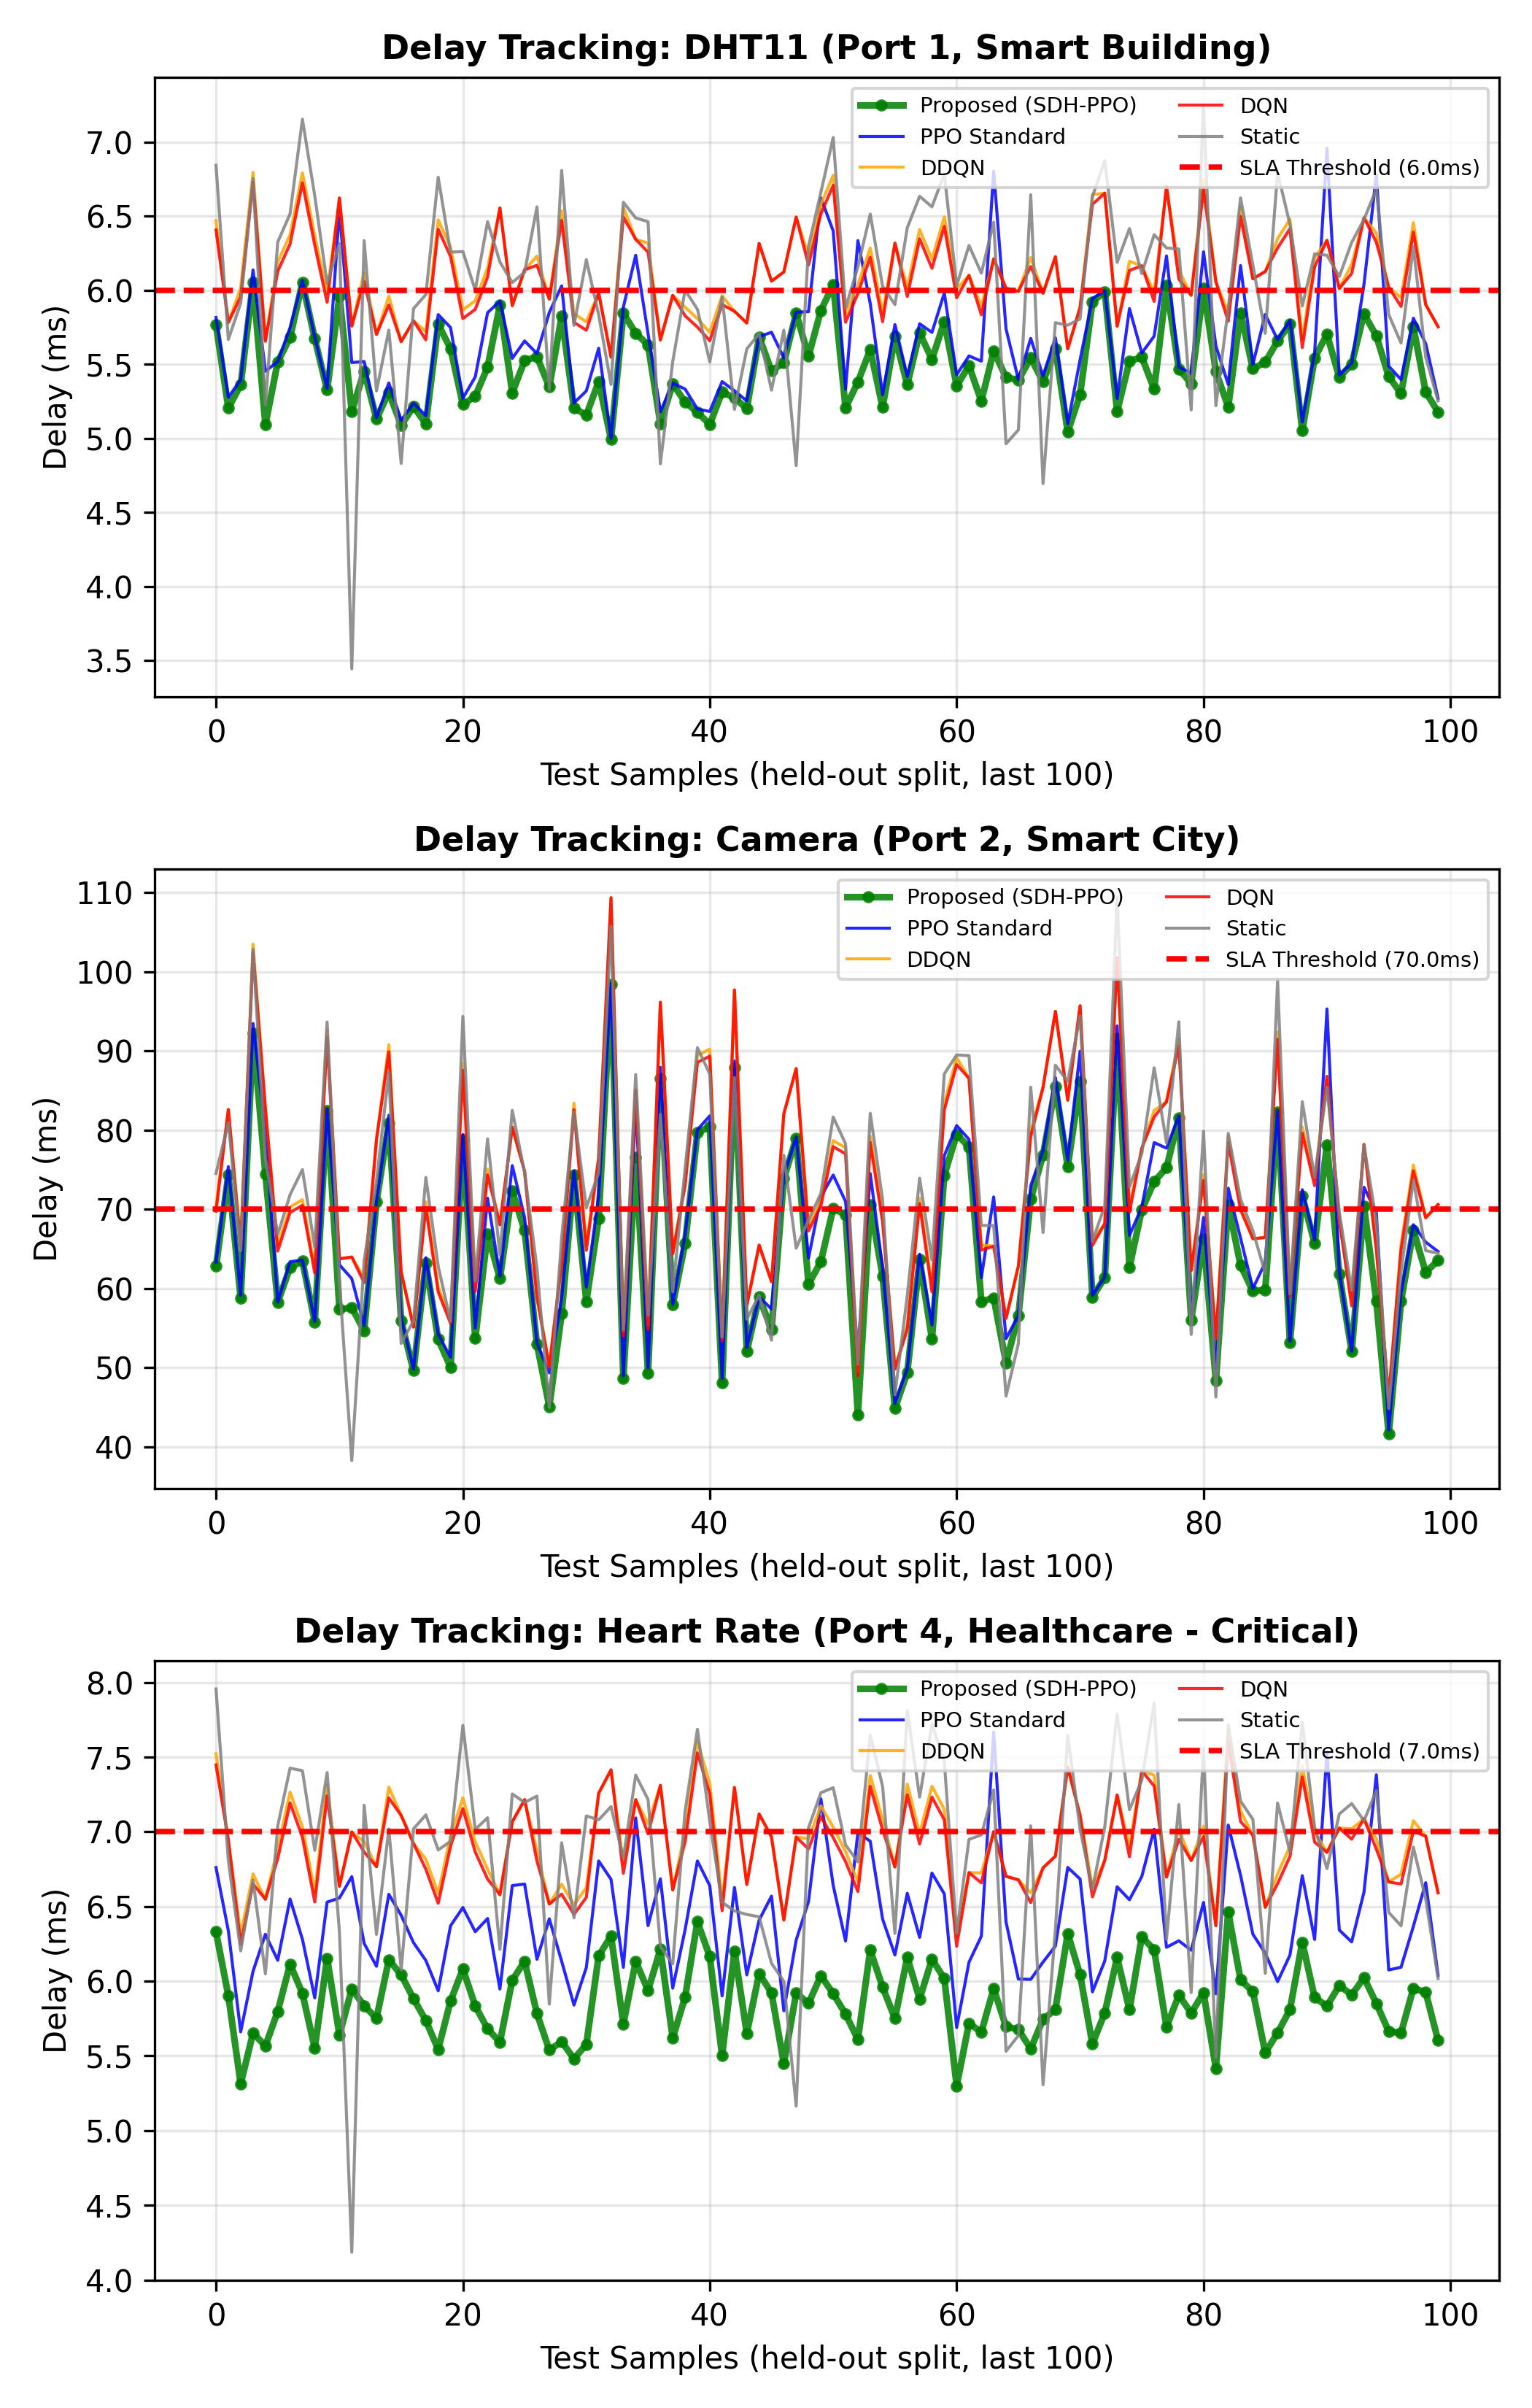
\includegraphics[width=\columnwidth]{figures/fig4_port_delay_track.png}
\caption{Port Delay Track.}
\label{fig:4}
\end{figure}


\begin{figure}[htbp]
\centering
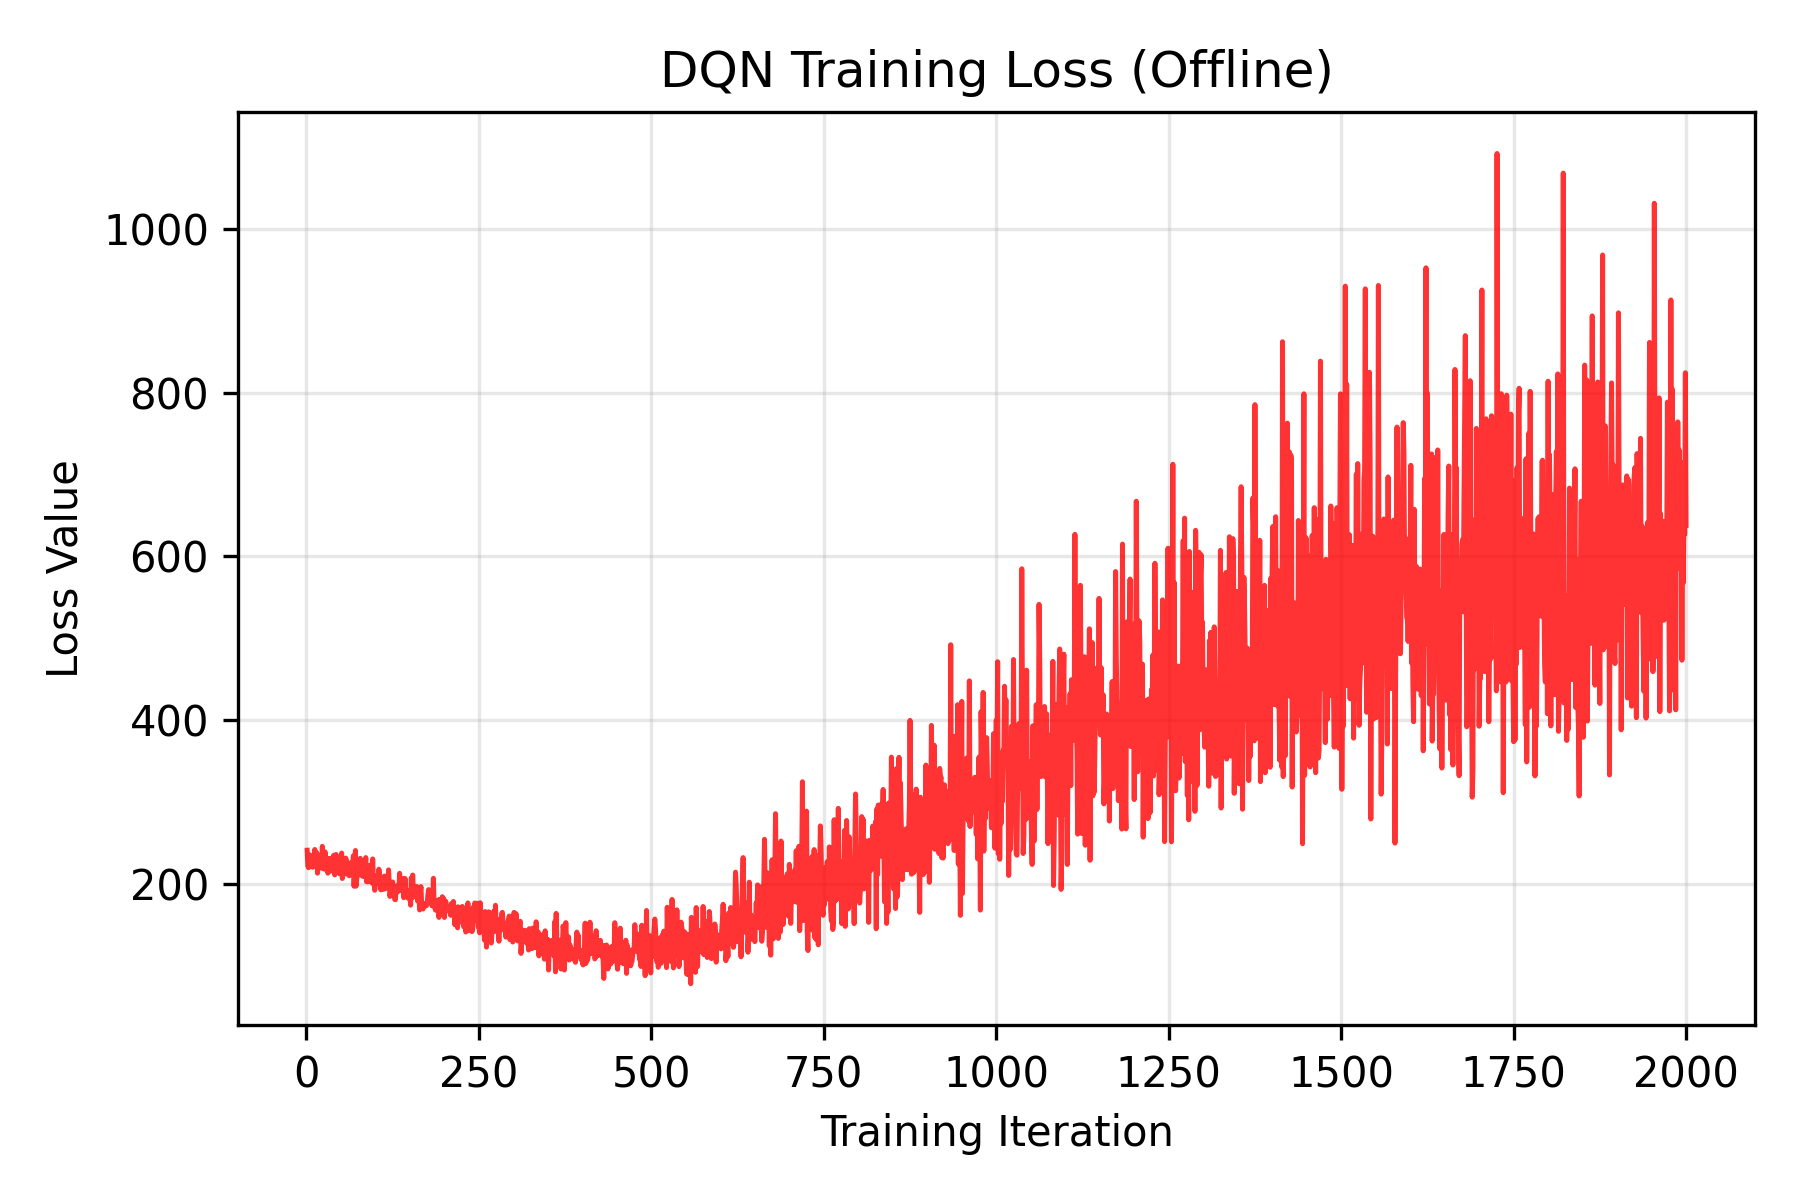
\includegraphics[width=\columnwidth]{figures/fig5_dqn_convergence.png}
\caption{DQN Convergence \& Reward Progress.}
\label{fig:5}
\end{figure}


\begin{figure}[htbp]
\centering
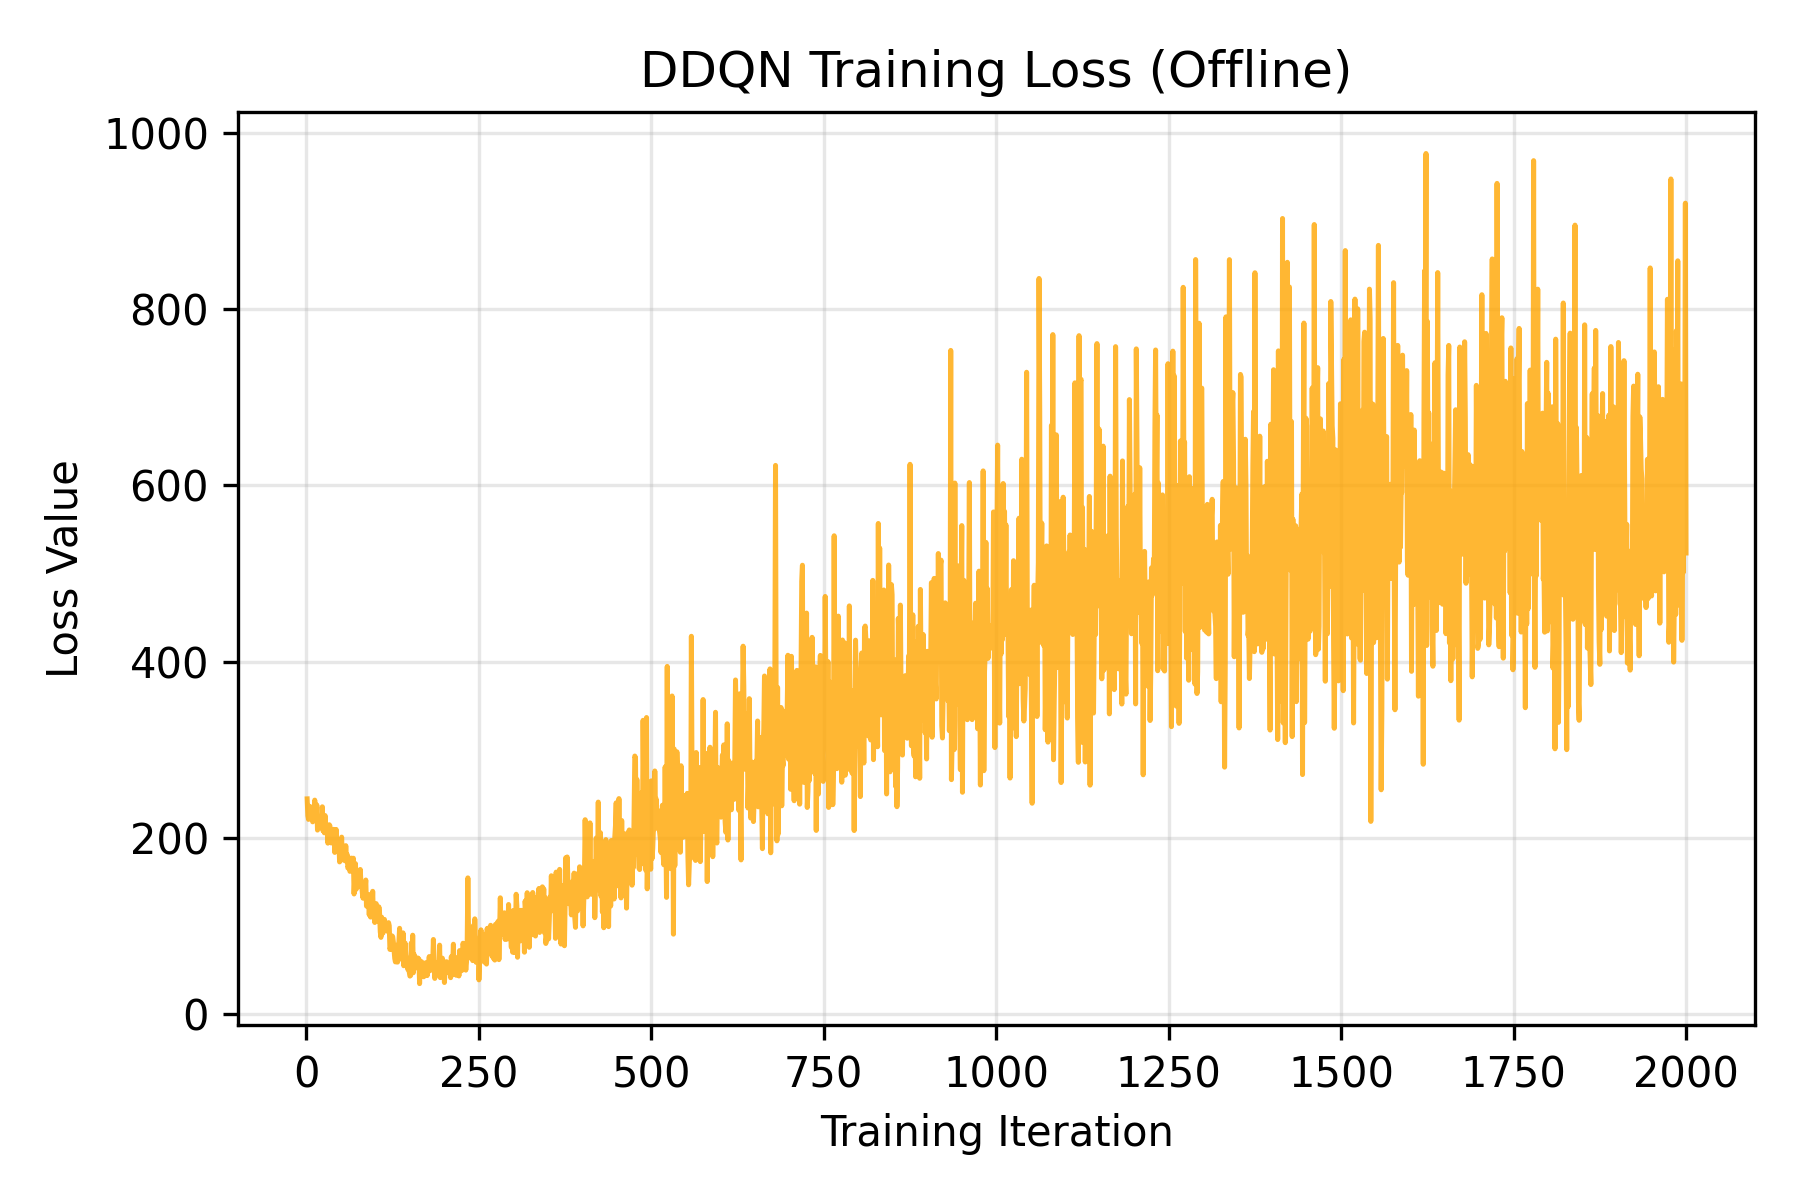
\includegraphics[width=\columnwidth]{figures/fig6_ddqn_convergence.png}
\caption{DDQN Convergence \& Reward Progress.}
\label{fig:6}
\end{figure}


\begin{table*}[t]
\centering
\caption{Performance Comparison Across Different Resource Allocation Algorithms}
\label{tab:3}
\begin{tabular}{lccccccc}
\toprule
Algorithm & P1 Avg (ms) & P1 Viol (\%) & P2 Avg (ms) & P2 Viol (\%) & P4 Avg (ms) & P4 Viol (\%) & Total Viol (\%) \\
\midrule
Proposed & 11.98 & 49.4 & 9.50 & 32.5 & 2.71 & 0.0 & 27.3 \\
PPO Standard & 11.99 & 49.4 & 9.52 & 33.6 & 3.36 & 42.0 & 41.6 \\
Double DQN & 12.00 & 49.7 & 9.48 & 31.9 & 3.33 & 39.3 & 40.3 \\
DQN & 12.04 & 51.8 & 9.50 & 33.5 & 3.34 & 39.5 & 41.6 \\
Static (Heuristic) & 11.98 & 48.9 & 9.49 & 32.8 & 3.76 & 67.2 & 49.6 \\
\bottomrule
\end{tabular}
\end{table*}

The comparative results of the proposed SDH-PPO framework against other baseline algorithms are summarized in Table 3. In this evaluation, lower numerical values for both average latency (ms) and violation percentage (\%) are indicative of superior performance, as they represent a reduction in Service Level Agreement (SLA) breaches and more efficient resource management. As observed in the table, the proposed framework consistently outperforms both traditional reinforcement learning models and the static heuristic baseline. Notably, our approach achieves the lowest total violation rate of 27.3\%, marking a significant improvement over the Static Heuristic (\(49.6\%\)) and standard PPO (41.6\%). The most substantial performance gain is evident in Priority 4 (P4) traffic, where the proposed model achieves a 0.0\% violation rate and an average latency of only 2.71 ms. These results demonstrate that the proposed SDH-PPO framework is more adept at prioritizing critical traffic and maintaining SLA compliance across diverse network slicing scenarios compared to existing methodologies.

\begin{figure}[htbp]
\centering
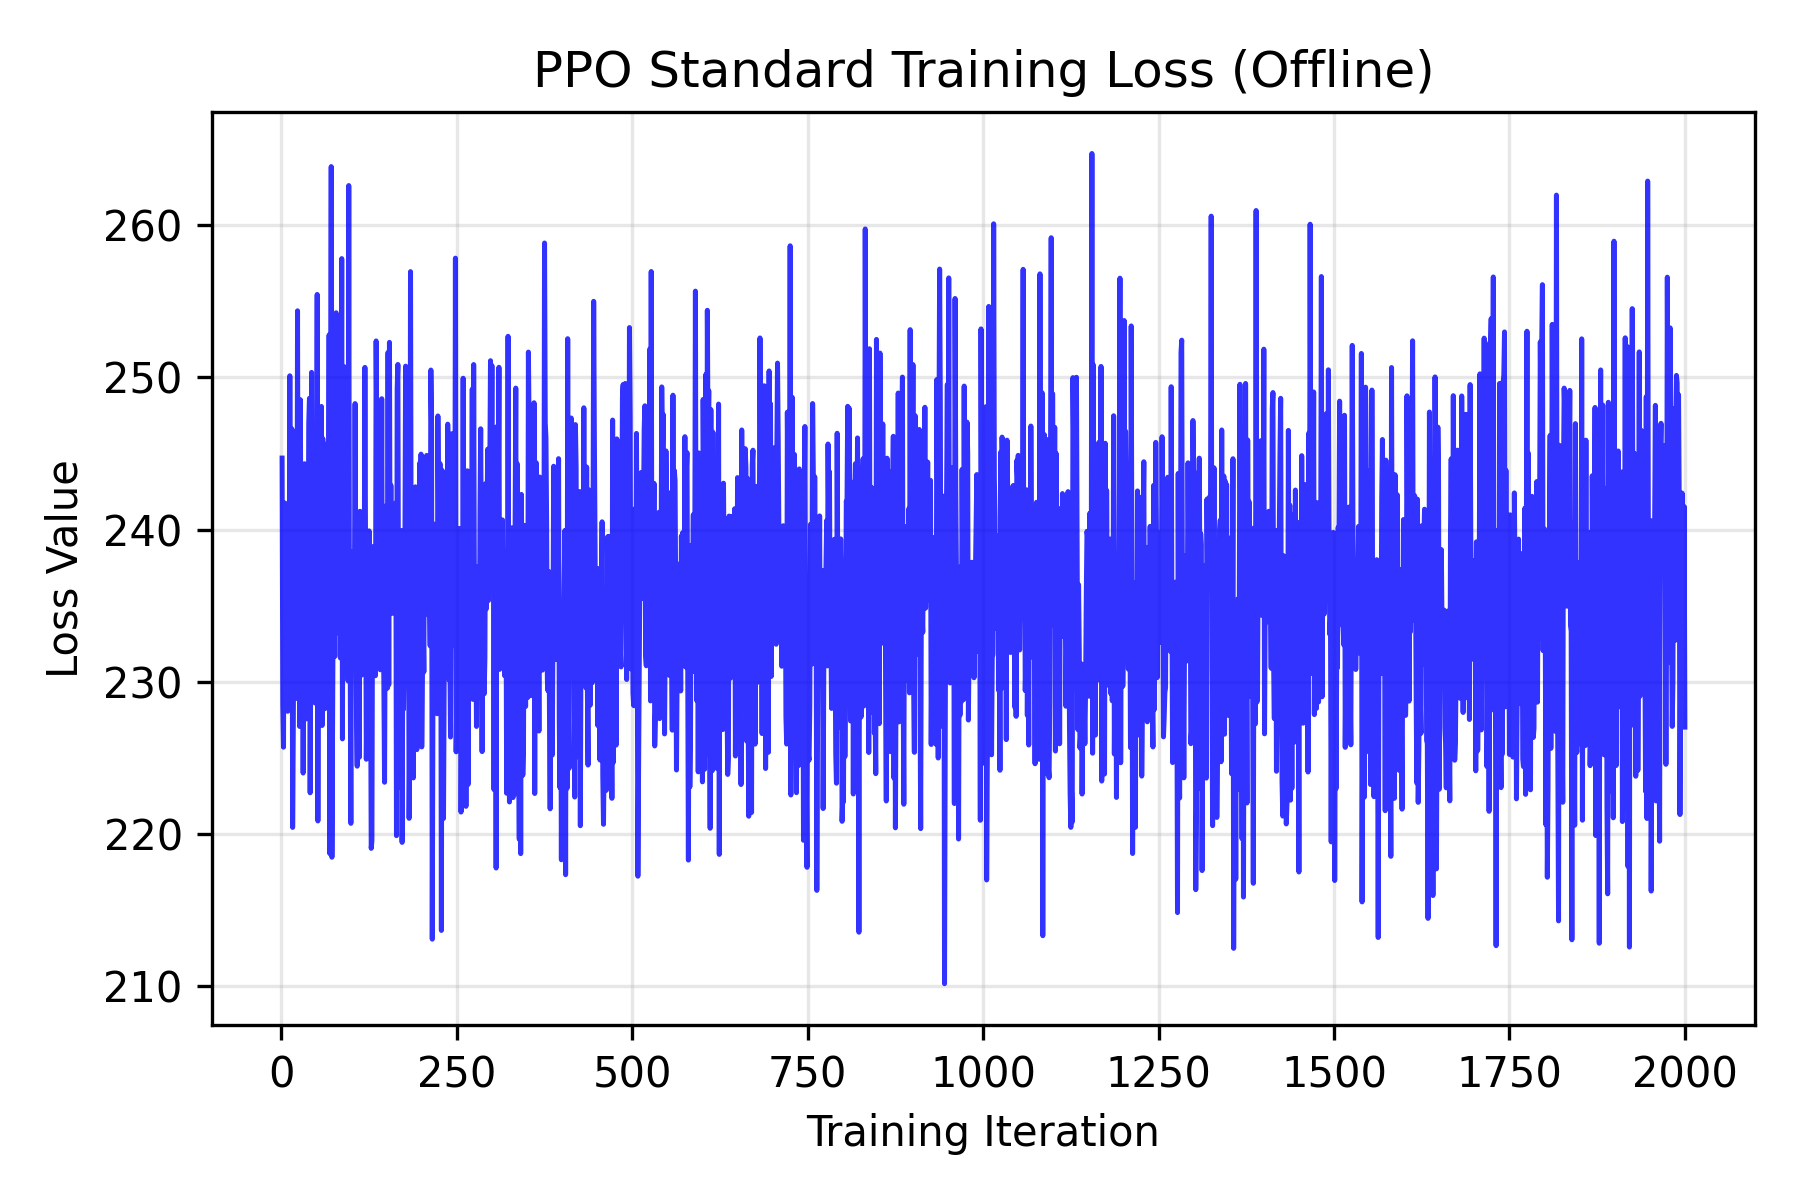
\includegraphics[width=\columnwidth]{figures/fig7_ppo_convergence.png}
\caption{PPO Convergence \& Reward Progress.}
\label{fig:7}
\end{figure}


\begin{figure}[htbp]
\centering
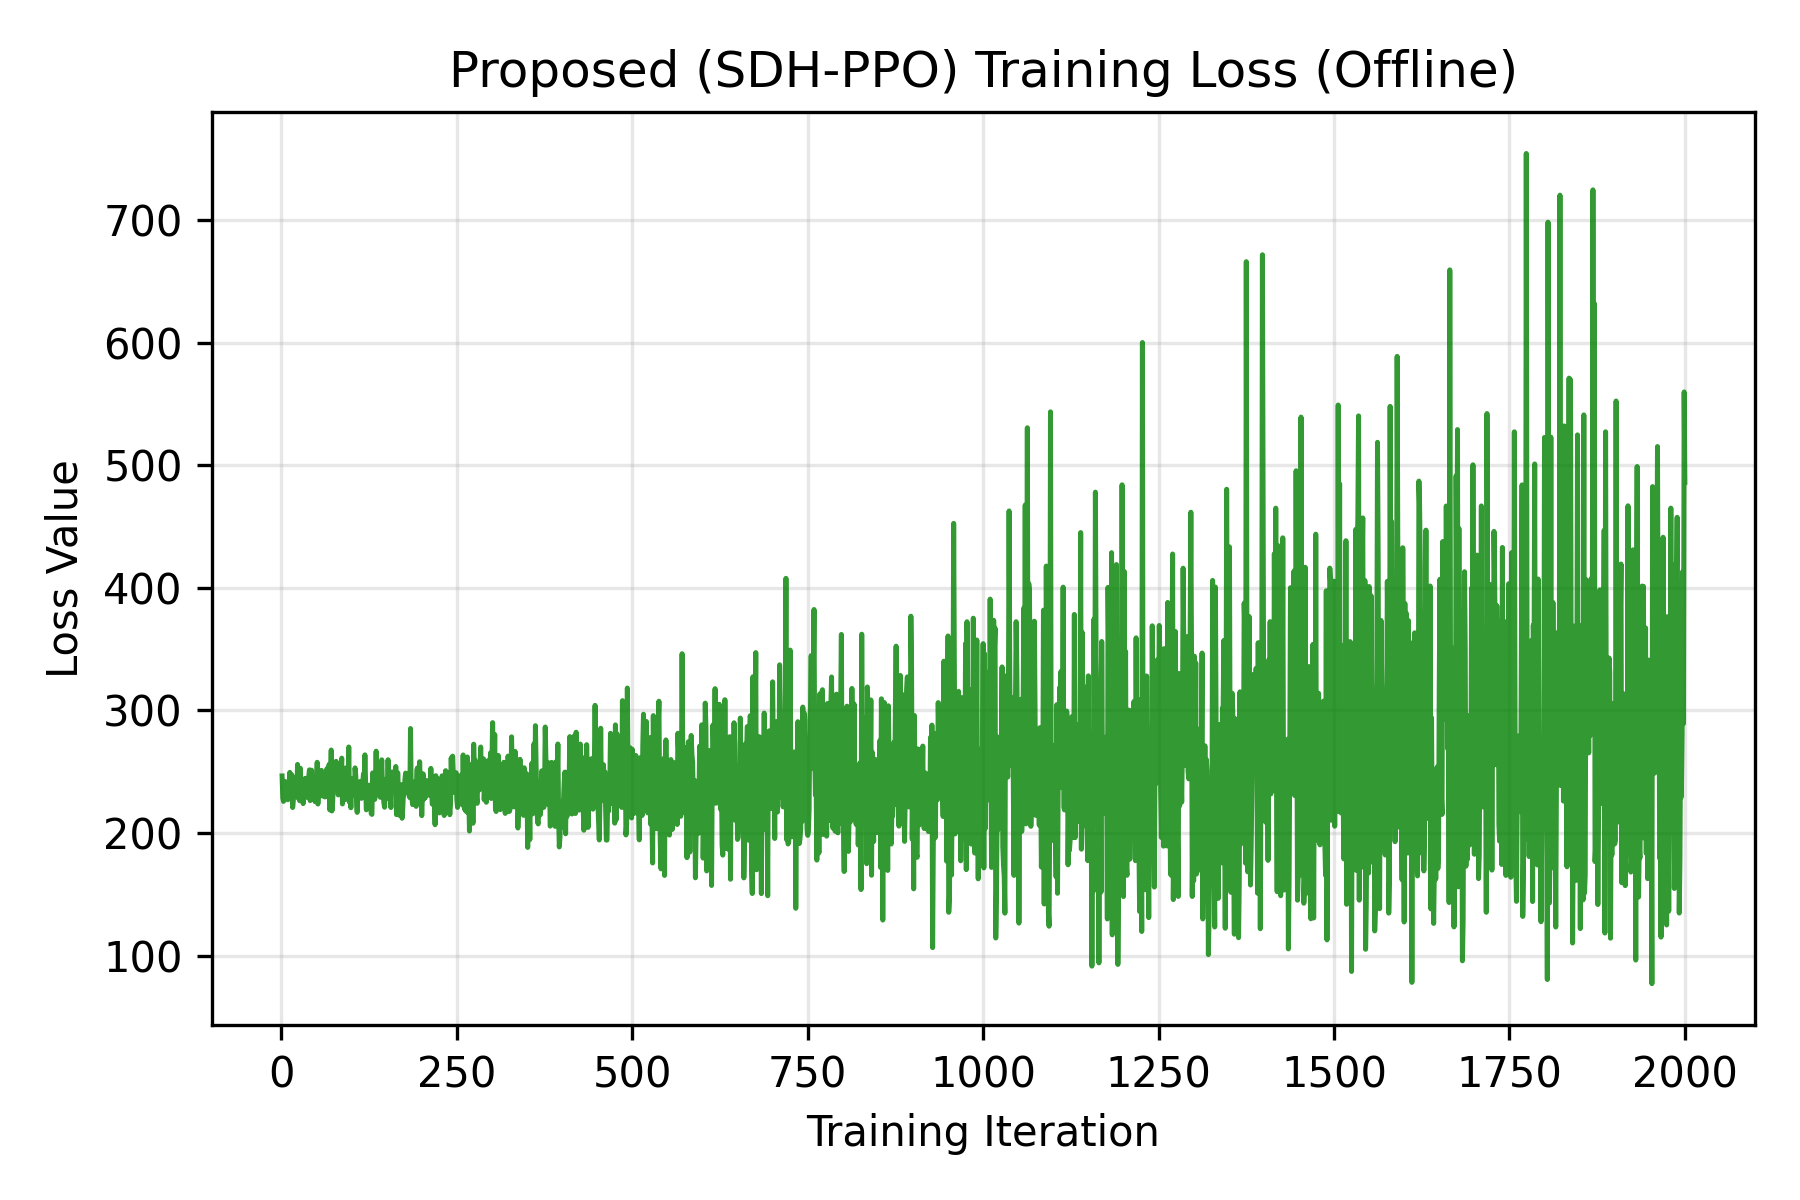
\includegraphics[width=\columnwidth]{figures/fig8_sdh_ppo_convergence.png}
\caption{SDH-PPO (Proposed) Convergence \& Reward Progress.}
\label{fig:8}
\end{figure}


\section{V. Conclusions}\label{v.-conclusions}

This research has presented the SDH-PPO framework as an autonomous resource orchestration strategy to address the operational challenges in multi-tenant SDN-based IoT environments. By integrating WGAN-GP-based data augmentation, the proposed framework successfully encapsulated latent traffic probability distributions, which significantly enhanced the learning agent\textquotesingle s generalization capabilities across various network slicing scenarios. Experimental results demonstrate that the SDH-PPO framework consistently outperforms baseline methodologies, achieving a superior total violation rate of 27.3\%, representing a performance improvement of more than 47.6\% over standard implementations. Most notably, the framework achieved a 0.0\% violation rate for critical Priority 4 (P4) traffic with a minimal average latency of 2.71 ms, ensuring rigorous adherence to Service Level Agreements (SLAs) for sensitive telemetry. Although the proposed model requires approximately twice the training epochs to converge compared to traditional models, the resulting policy exhibits exceptional stability and robustness in its reward acquisition process. Ultimately, these findings validate the efficacy of the SDH-PPO framework as a reliable and adaptive solution for dynamic resource management in next-generation IoT infrastructures.